\section{Preventivo}
\label{preventivo}
Per ogni periodo individuato nella sezione \S\ref{pianificazione} relativa alla pianificazione, si espone un prospetto orario dove sono raccolte le ore che ciascun membro deve svolgere per ruolo.\\Viene successivamente mostrato un prospetto economico che riassume i costi sostenuti per ciascun ruolo.\\
Per agevolare la lettura delle tabelle, se un membro del gruppo non ha ricoperto un certo ruolo verrà inserito il simbolo \textbf{-} per indicarne l'assenza.\\Si è poi pensato di utilizzare le seguenti sigle per identificare i ruoli:
\begin{itemize}
\item \textbf{Re:} {\Responsabile};
\item \textbf{Am:} {\Amministratore};
\item \textbf{An:} \textit{Analista};
\item \textbf{Pt:} \textit{Progettista};
\item \textbf{Pr:} \textit{Programmatore};
\item \textbf{Ve:} \textit{Verificatore}.
\end{itemize}
\newpage

\subsection{Periodo di analisi}
\subsubsection{Prospetto orario}
In questo periodo, ogni componente del gruppo rivestirà i seguenti ruoli:
\begin{table}[H]
	\begin{center}
		\begin{tabular}{ |c c c c c c c c|}
		\rowcolor{darkblue} 
		\textcolor{white}{\textbf{Nominativo}} & \textcolor{white}{\textbf{Re}} & \textcolor{white}{\textbf{Am}} & \textcolor{white}{\textbf{An}} & \textcolor{white}{\textbf{Pt}} & \textcolor{white}{\textbf{Pr}} & \textcolor{white}{\textbf{Ve}} & \textcolor{white}{\textbf{Ore Complessive}}\\ \hline
		\BL 	& - 	& 6 	& 16 	& - 	& - 	& 8 	& 30 \\ \hline
		\FF 	& - 	& 5 	& 15 	& - 	& - 	& 10 	& 30 \\ \hline
		\MM		& 15	& - 	& 10 	& - 	& - 	& 5 	& 30 \\ \hline
		\PC		& 5 	& 4 	& 10 	& - 	& - 	& 11	& 30 \\ \hline
		\TG 	& - 	& 15	& 10 	& - 	& - 	& 5 	& 30 \\ \hline
		\TL 	& 4 	& 5 	& 16 	& - 	& - 	& 5 	& 30 \\ \hline
		\VD 	& - 	& -  	& 12 	& - 	& - 	& 18 	& 30 \\ \hline
		\textbf{Ore totali} & \textbf{24} & \textbf{35} & \textbf{89} & \textbf{-} & \textbf{-} & \textbf{62} & \textbf{210} \\ \hline
		\end{tabular}
	\caption{Distribuzione delle ore nel periodo di analisi}
	\end{center}
\end{table}
I dati ottenuti vengono riassunti nel seguente istogramma:
\begin{figure}[H]
    \centering
    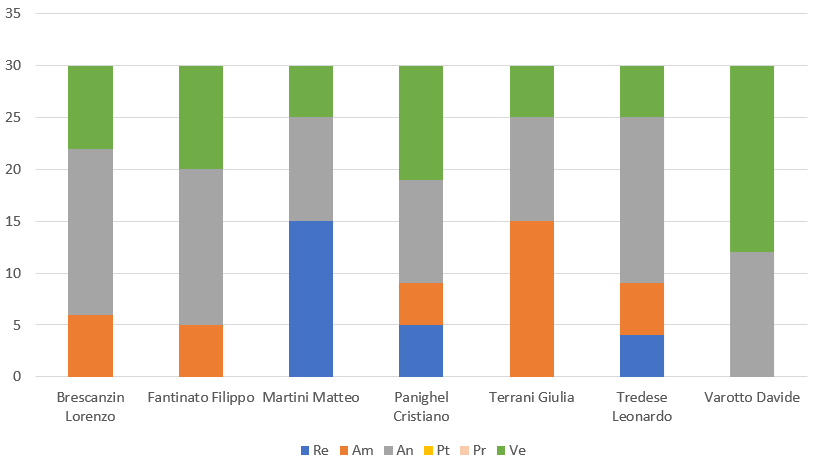
\includegraphics[scale = 0.70]{Immagini/AnalisiIsto.png}
    \caption{Istogramma della ripartizione delle ore per ruolo in analisi}
    \label{fig:istogramma ripartizione ore, periodo di Analisi}
\end{figure}
\newpage
\subsubsection{Prospetto economico}
Il costo per ogni ruolo è il seguente:
\begin{table}[H]
	\begin{center}
		\begin{tabular}{ |c c c| }
		\rowcolor{darkblue} 
		\textcolor{white}{\textbf{Ruolo}} & \textcolor{white}{\textbf{Ore}} & \textcolor{white}{\textbf{Costo in €}}\\ \hline
		{\Responsabile} 			& 24 	& 720 \\ \hline
		{\Amministratore} 			& 35 	& 700 \\ \hline
		\textit{Analista} 			& 89 	& 2225 \\ \hline
		\textit{Progettista} 		& - 	& - \\ \hline
		\textit{Programmatore}  	& - 	& - \\ \hline
		\textit{Verificatore} 		& 62 	& 930 \\ \hline
		\textbf{Totale} 			& \textbf{210} & \textbf{4575} \\ \hline
		\end{tabular}
	\caption{Prospetto dei costi per ruoli nel periodo di analisi}
	\end{center}
\end{table}
Il seguente grafico a torta riassume i dati ottenuti:
\begin{figure}[H]
    \centering
    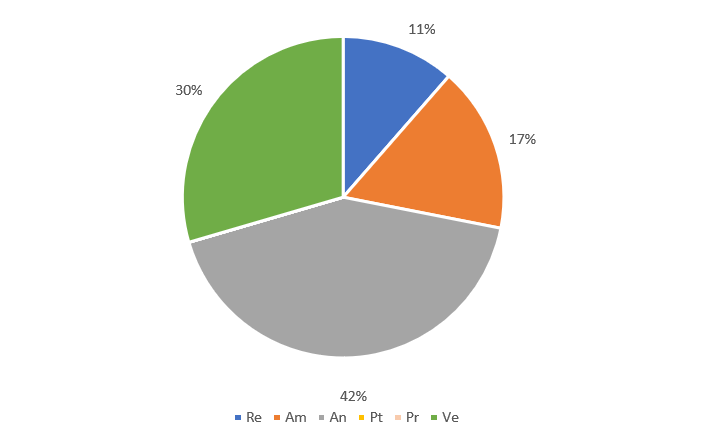
\includegraphics[scale = 0.75]{Immagini/AnalisiTorta.png}
    \caption{Areogramma ripartizione ore, periodo di analisi}
    \label{fig:Areogramma ripartizione ore, periodo di Analisi}
\end{figure}
\newpage

\subsection{Periodo di consolidamento dei requisiti}
\subsubsection{Prospetto orario}
Durante il periodo di consolidamento dei requisiti viene effettuata la seguente distribuzione oraria:
\begin{table}[H]
	\begin{center}
		\begin{tabular}{ |c c c c c c c c| }
		\rowcolor{darkblue} 
		\textcolor{white}{\textbf{Nominativo}} & \textcolor{white}{\textbf{Re}} & \textcolor{white}{\textbf{Am}} & \textcolor{white}{\textbf{An}} & \textcolor{white}{\textbf{Pt}} & \textcolor{white}{\textbf{Pr}} & \textcolor{white}{\textbf{Ve}} & \textcolor{white}{\textbf{Ore Complessive}} \\ \hline
		\BL 	& - 	& 3  	& - 	& 3 	& - 	& - 	& 6 \\ \hline
		\FF 	& - 	& 3  	& 3 	& - 	& - 	& -  	& 6 \\ \hline
		\MM 	& -  	& -  	& 2 	& - 	& - 	& 4  	& 6 \\ \hline
		\PC 	& - 	& -  	& 4 	& 2 	& - 	& - 	& 6 \\ \hline
		\TG 	& 2  	& - 	& 4 	& - 	& - 	& - 	& 6 \\ \hline
		\TL 	& 3  	& - 	& - 	& - 	& - 	& 3 	& 6 \\ \hline
		\VD 	& -  	& -  	& 4 	& 2 	& - 	& -  	& 6 \\ \hline
		\textbf{Ore totali} & \textbf{5} & \textbf{6} & \textbf{17} & \textbf{7} & \textbf{-} & \textbf{7} & \textbf{42} \\ \hline
		\end{tabular}
	\caption{Distribuzione delle ore nel periodo di consolidamento dei requisiti}
	\end{center}
\end{table}
I dati ottenuti vengono riassunti nel seguente istogramma:
\begin{figure}[H]
    \centering
    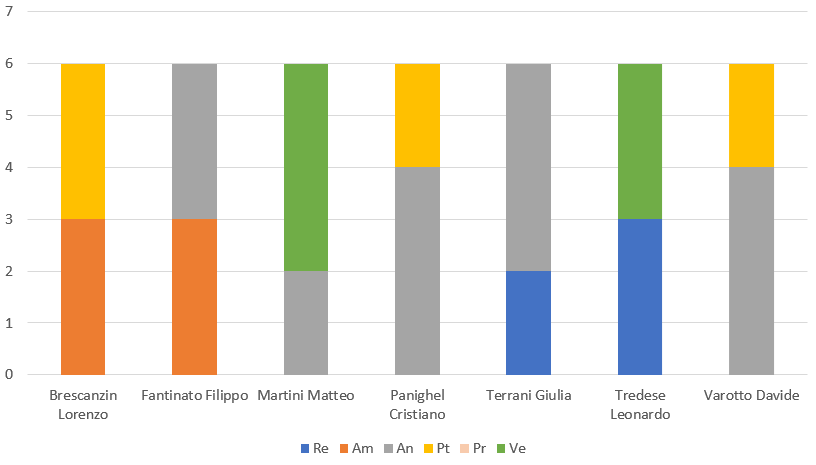
\includegraphics[scale = 0.70]{Immagini/ConsolidamentoIsto.png}
    \caption{Istogramma della ripartizione delle ore per ruolo in consolidamento dei requisiti}
    \label{fig:istogramma ripartizione ore, periodo di Consolidamento dei Requisiti}
\end{figure}
\newpage
\subsubsection{Prospetto economico}
Il costo per ogni ruolo è il seguente:
\begin{table}[H]
	\begin{center}
		\begin{tabular}{ |c c c|}
		\rowcolor{darkblue} 
		\textcolor{white}{\textbf{Ruolo}} & \textcolor{white}{\textbf{Ore}} & \textcolor{white}{\textbf{Costo in €}}\\ \hline
		{\Responsabile} 			& 5 	& 150 \\ \hline
		{\Amministratore} 			& 6 	& 120 \\ \hline
		\textit{Analista} 			& 17 	& 425 \\ \hline
		\textit{Progettista} 		& 7 	& 154 \\ \hline
		\textit{Programmatore}  	& - 	& - \\ \hline
		\textit{Verificatore} 		& 7 	& 105 \\ \hline
		\textbf{Totale} 			& \textbf{42} & \textbf{954} \\ \hline
		\end{tabular}
	\caption{Prospetto dei costi per ruoli nel periodo di consolidamento dei requisiti}
	\end{center}
\end{table}
Il seguente grafico a torta riassume i dati ottenuti:
\begin{figure}[H]
    \centering
    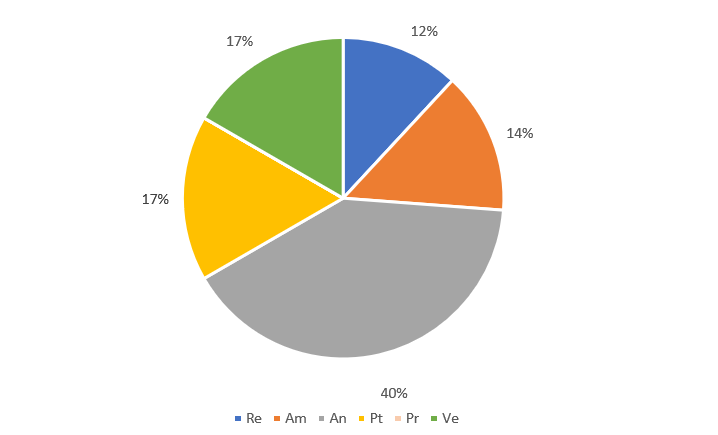
\includegraphics[scale = 0.75]{Immagini/ConsolidamentoTorta.png}
    \caption{Areogramma della ripartizione di ore per ruolo in consolidamento dei requisiti}
    \label{fig:Areogramma ripartizione ore, periodo di Consolidamento dei Requisiti}
\end{figure}
\newpage

\subsection{Periodo di progettazione architetturale}\label{PreventiviPArchitetturale}
\subsubsection{Prospetto orario}
In questo periodo la distribuzione oraria è la seguente:
\begin{table}[H]
	\begin{center}
		\begin{tabular}{ |c c c c c c c c| }
		\rowcolor{darkblue} 
		\textcolor{white}{\textbf{Nominativo}} & \textcolor{white}{\textbf{Re}} & \textcolor{white}{\textbf{Am}} & \textcolor{white}{\textbf{An}} & \textcolor{white}{\textbf{Pt}} & \textcolor{white}{\textbf{Pr}} & \textcolor{white}{\textbf{Ve}} & \textcolor{white}{\textbf{Ore Complessive}} \\ \hline
	\BL 	& -  	& -  	& 8 	& 12 	& 3 	& 7 	& 30 \\ \hline
	\FF 	& 3  	& -  	& - 	& 16 	& 5 	& 6  	& 30 \\ \hline
	\MM 	& -  	& 3  	& 10 	& 8 	& 5 	& 4  	& 30 \\ \hline
	\PC 	& - 	& -  	& 10 	& - 	& 4 	& 16 	& 30 \\ \hline
	\TG 	& -  	& 3 	& 10 	& 13 	& - 	& 4 	& 30 \\ \hline
	\TL 	& 5  	& 6 	& - 	& - 	& 4 	& 15 	& 30 \\ \hline
	\VD 	& 10  	& 8  	& - 	& 12 	& - 	& -  	& 30 \\ \hline
	\textbf{Ore totali} & \textbf{18} & \textbf{20} & \textbf{38} & \textbf{61} & \textbf{21} & \textbf{52} & \textbf{210} \\ \hline
\end{tabular}
	\caption{Distribuzione delle ore nel periodo di progettazione architetturale}
	\end{center}
\end{table}
I dati ottenuti vengono riassunti nel seguente istogramma:
\begin{figure}[H]
    \centering
    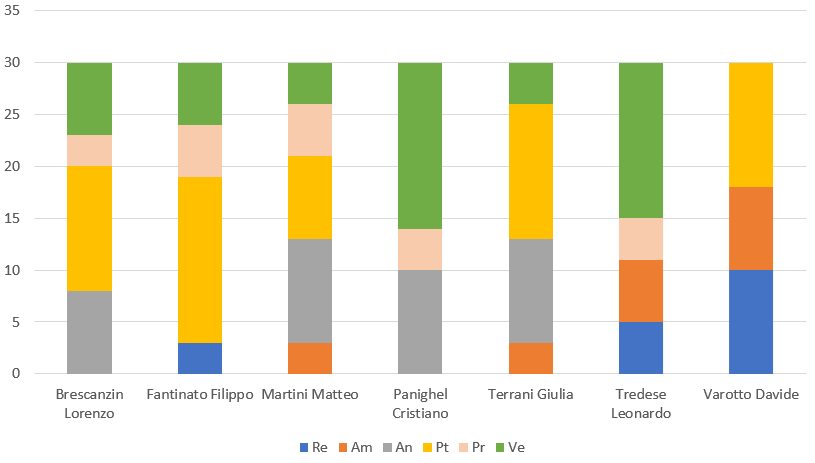
\includegraphics[scale = 0.70]{Immagini/ArchitetturaIsto.png}
    \caption{Istogramma della ripartizione delle ore per ruolo in progettazione architetturale}
    \label{fig:istogramma ripartizione ore, periodo di Progettazione Architetturale}
\end{figure}
\newpage
\subsubsection{Prospetto economico}
Il costo per ogni ruolo è il seguente:
\begin{table}[H]
	\begin{center}
		\begin{tabular}{ |c c c| }
		\rowcolor{darkblue} 
		\textcolor{white}{\textbf{Ruolo}} & \textcolor{white}{\textbf{Ore}} & \textcolor{white}{\textbf{Costo in €}}\\ \hline
	{\Responsabile} 			& 18 & 540 \\ \hline
	{\Amministratore} 			& 20 & 400 \\ \hline
	\textit{Analista} 			& 38 & 950 \\ \hline
	\textit{Progettista} 		& 61 & 1342\\ \hline
	\textit{Programmatore}  	& 21 & 315 \\ \hline
	\textit{Verificatore} 		& 52 & 780 \\ \hline
	\textbf{Totale} & \textbf{210} & \textbf{4327} \\ \hline
	\end{tabular}
	\caption{Prospetto dei costi per ruoli nel periodo di progettazione architetturale}
	\end{center}
\end{table}
Il seguente grafico a torta riassume i dati ottenuti:
\begin{figure}[H]
    \centering
    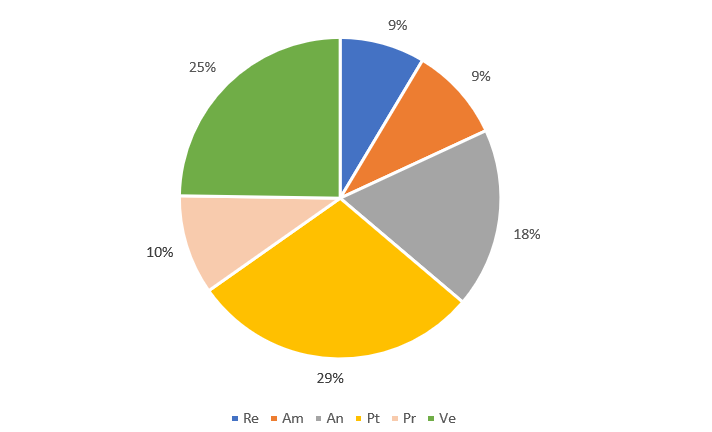
\includegraphics[scale = 0.75]{Immagini/ArchitetturaTorta.png}
    \caption{Areogramma della ripartizione di ore per ruolo in progettazione architetturale}
    \label{fig:Areogramma ripartizione ore, periodo di Progettazione Architetturale}
\end{figure}

\subsubsection{Specifica dei prospetti}
Per un maggiore controllo sul periodo di progettazione architetturale, vengono di seguito riportati i prospetti orari ed economici suddivisi per le attività individuate nella sezione \S\ref{progettazione_architetturale}.
\paragraph{Incremento e verifica documenti}
\paragraph*{Prospetto orario}
La distribuzione oraria è la seguente:
\begin{table}[H]
	\begin{center}
		\begin{tabular}{ |c c c c c c c c| }
			\rowcolor{darkblue} 
			\textcolor{white}{\textbf{Nominativo}} & \textcolor{white}{\textbf{Re}} & \textcolor{white}{\textbf{Am}} & \textcolor{white}{\textbf{An}} & \textcolor{white}{\textbf{Pt}} & \textcolor{white}{\textbf{Pr}} & \textcolor{white}{\textbf{Ve}} & \textcolor{white}{\textbf{Ore Complessive}} \\ \hline
			\BL 	& -  	& -  	& 5 	& - 	& - 	& 4 	& 9 \\ \hline
			\FF 	& 3  	& -  	& - 	& - 	& - 	& 6  	& 9 \\ \hline
			\MM 	& -  	& 2  	& 6 	& -		& - 	& 1  	& 9 \\ \hline
			\PC 	& - 	& -  	& 6 	& - 	& - 	& 3 	& 9 \\ \hline
			\TG 	& -  	& 2 	& 6 	& - 	& - 	& 1 	& 9 \\ \hline
			\TL 	& 2  	& 4 	& - 	& - 	& - 	& 3 	& 9 \\ \hline
			\VD 	& 4  	& 5  	& - 	& - 	& - 	& -  	& 9 \\ \hline
			\textbf{Ore totali} & \textbf{9} & \textbf{13} & \textbf{23} & \textbf{0} & \textbf{0} & \textbf{18} & \textbf{63} \\ \hline
		\end{tabular}
		\caption{Distribuzione delle ore}
	\end{center}
\end{table}
\paragraph*{Prospetto economico}
Il costo per ogni ruolo è il seguente:
\begin{table}[H]
	\begin{center}
		\begin{tabular}{ |c c c| }
			\rowcolor{darkblue} 
			\textcolor{white}{\textbf{Ruolo}} & \textcolor{white}{\textbf{Ore}} & \textcolor{white}{\textbf{Costo in €}}\\ \hline
			{\Responsabile} 			& 9 & 270 \\ \hline
			{\Amministratore} 			& 13 & 260 \\ \hline
			\textit{Analista} 			& 23 & 575 \\ \hline
			\textit{Progettista} 		& - & - \\ \hline
			\textit{Programmatore}  	& - & - \\ \hline
			\textit{Verificatore} 		& 18 & 270 \\ \hline
			\textbf{Totale} & \textbf{63} & \textbf{1375} \\ \hline
		\end{tabular}
		\caption{Prospetto dei costi per ruoli}
	\end{center}
\end{table}

\paragraph{\glo{TB} e \glo{PoC}- Incremento 1}
\paragraph*{Prospetto orario}
La distribuzione oraria è la seguente:
\begin{table}[H]
	\begin{center}
		\begin{tabular}{ |c c c c c c c c| }
			\rowcolor{darkblue} 
			\textcolor{white}{\textbf{Nominativo}} & \textcolor{white}{\textbf{Re}} & \textcolor{white}{\textbf{Am}} & \textcolor{white}{\textbf{An}} & \textcolor{white}{\textbf{Pt}} & \textcolor{white}{\textbf{Pr}} & \textcolor{white}{\textbf{Ve}} & \textcolor{white}{\textbf{Ore Complessive}} \\ \hline
			\BL 	& -  	& -  	& 2 	& 9 	& - 	& - 	& 11 \\ \hline
			\FF 	& -  	& -  	& - 	& 8 	& 3 	& -  	& 11 \\ \hline
			\MM 	& -  	& 1  	& 2 	& 4 	& 3 	& 1  	& 11 \\ \hline
			\PC 	& - 	& -  	& 2 	& - 	& 3 	& 6 	& 11 \\ \hline
			\TG 	& -  	& - 	& 4 	& 5 	& - 	& 2 	& 11 \\ \hline
			\TL 	& 2  	& 2 	& - 	& - 	& 3 	& 4 	& 11 \\ \hline
			\VD 	& 3  	& 2  	& - 	& 6 	& - 	& -  	& 11 \\ \hline
			\textbf{Ore totali} & \textbf{5} & \textbf{5} & \textbf{10} & \textbf{32} & \textbf{12} & \textbf{13} & \textbf{77} \\ \hline
		\end{tabular}
		\caption{Distribuzione delle ore }
	\end{center}
\end{table}
\paragraph*{Prospetto economico}
Il costo per ogni ruolo è il seguente:
 \begin{table}[H]
 	\begin{center}
 		\begin{tabular}{ |c c c| }
 			\rowcolor{darkblue} 
 			\textcolor{white}{\textbf{Ruolo}} & \textcolor{white}{\textbf{Ore}} & \textcolor{white}{\textbf{Costo in €}}\\ \hline
 			{\Responsabile} 			& 5 & 150 \\ \hline
 			{\Amministratore} 			& 5 & 100 \\ \hline
 			\textit{Analista} 			& 10 & 250 \\ \hline
 			\textit{Progettista} 		& 32 & 704\\ \hline
 			\textit{Programmatore}  	& 12 & 180 \\ \hline
 			\textit{Verificatore} 		& 13 & 195 \\ \hline
 			\textbf{Totale} & \textbf{77} & \textbf{1579} \\ \hline
 		\end{tabular}
 		\caption{Prospetto dei costi per ruoli}
 	\end{center}
 \end{table}
\paragraph{TB e PoC - Incremento 2}
\paragraph*{Prospetto orario}
In questo periodo la distribuzione oraria è la seguente:
\begin{table}[H]
	\begin{center}
		\begin{tabular}{ |c c c c c c c c| }
			\rowcolor{darkblue} 
			\textcolor{white}{\textbf{Nominativo}} & \textcolor{white}{\textbf{Re}} & \textcolor{white}{\textbf{Am}} & \textcolor{white}{\textbf{An}} & \textcolor{white}{\textbf{Pt}} & \textcolor{white}{\textbf{Pr}} & \textcolor{white}{\textbf{Ve}} & \textcolor{white}{\textbf{Ore Complessive}} \\ \hline
			\BL 	& -		& -  	& 1 	& 3 	& 3 	& 3		& 10 \\ \hline
			\FF 	& -  	& -  	& - 	& 8 	& 2 	& -  	& 10 \\ \hline
			\MM 	& -  	& -  	& 2 	& 4		& 2 	& 2  	& 10 \\ \hline
			\PC 	& - 	& -  	& 2 	& - 	& 1 	& 7 	& 10 \\ \hline
			\TG 	& -  	& 1 	& - 	& 8		& - 	& 1 	& 10 \\ \hline
			\TL 	& 1  	& - 	& - 	& - 	& 1 	& 8 	& 10 \\ \hline
			\VD 	& 3  	& 1  	& - 	& 6 	& - 	& -  	& 10 \\ \hline
			\textbf{Ore totali} & \textbf{4} & \textbf{2} & \textbf{5} & \textbf{29} & \textbf{9} & \textbf{21} & \textbf{70} \\ \hline
		\end{tabular}
		\caption{Distribuzione delle ore}
	\end{center}
\end{table}
\paragraph*{Prospetto economico}
Il costo per ogni ruolo è il seguente:
\begin{table}[H]
	\begin{center}
		\begin{tabular}{ |c c c| }
			\rowcolor{darkblue} 
			\textcolor{white}{\textbf{Ruolo}} & \textcolor{white}{\textbf{Ore}} & \textcolor{white}{\textbf{Costo in €}}\\ \hline
			{\Responsabile} 			& 4 & 120 \\ \hline
			{\Amministratore} 			& 2 & 40 \\ \hline
			\textit{Analista} 			& 5 & 125 \\ \hline
			\textit{Progettista} 		& 29 & 638\\ \hline
			\textit{Programmatore}  	& 9 & 135 \\ \hline
			\textit{Verificatore} 		& 21 & 315 \\ \hline
			\textbf{Totale} & \textbf{70} & \textbf{1373} \\ \hline
		\end{tabular}
		\caption{Prospetto dei costi per ruoli}
	\end{center}
\end{table}

\newpage
\subsection{Periodo di progettazione di dettaglio e codifica}
\subsubsection{Prospetto orario}
In questo periodo la distribuzione oraria è la seguente:
\begin{table}[H]
	\begin{center}
		\begin{tabular}{ |c c c c c c c c| }
		\rowcolor{darkblue} 
		\textcolor{white}{\textbf{Nominativo}} & \textcolor{white}{\textbf{Re}} & \textcolor{white}{\textbf{Am}} & \textcolor{white}{\textbf{An}} & \textcolor{white}{\textbf{Pt}} & \textcolor{white}{\textbf{Pr}} & \textcolor{white}{\textbf{Ve}} & \textcolor{white}{\textbf{Ore Complessive}} \\ \hline
		\BL 	& 4  	& -  	& - 	& 15 	& 21 	& 10 	& 50 \\ \hline
		\FF 	& -  	& -  	& - 	& 30 	& 20 	& -  	& 50 \\ \hline
		\MM 	& -  	& 8  	& - 	& 15 	& 15 	& 12 	& 50 \\ \hline
		\PC 	& 5 	& 4  	& - 	& 11 	& 18 	& 12 	& 50 \\ \hline
		\TG 	& 5  	& 2		& - 	& 6 	& 20 	& 17 	& 50 \\ \hline
		\TL 	& -  	& - 	& - 	& 15 	& 20 	& 15 	& 50 \\ \hline
		\VD 	& 4  	& 4  	& - 	& 12 	& 20 	& 10 	& 50 \\ \hline
		\textbf{Ore totali} & \textbf{18} & \textbf{18} & \textbf{-} & \textbf{104} & \textbf{134} & \textbf{76} & \textbf{350} \\ \hline
		\end{tabular}
	\caption{Distribuzione delle ore nel periodo di progettazione di dettaglio e codifica}
	\end{center}
\end{table}
I dati ottenuti vengono riassunti nel seguente istogramma:
\begin{figure}[H]
    \centering
    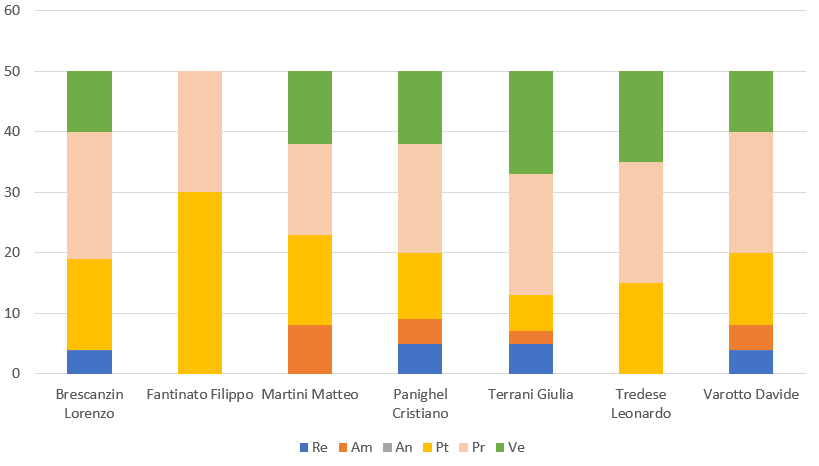
\includegraphics[scale = 0.70]{Immagini/DettaglioIsto.png}
    \caption{Istogramma della ripartizione delle ore per ruolo in progettazione di dettaglio e codifica}
    \label{fig:istogramma ripartizione ore, periodo di Progettazione di Dettaglio e Codifica}
\end{figure}
\newpage
\subsubsection{Prospetto economico}
Il costo per ogni ruolo è il seguente:
\begin{table}[H]
	\begin{center}
		\begin{tabular}{ |c c c| }
		\rowcolor{darkblue} 
		\textcolor{white}{\textbf{Ruolo}} & \textcolor{white}{\textbf{Ore}} & \textcolor{white}{\textbf{Costo in €}}\\ \hline
		{\Responsabile} 			& 18 	& 540 \\ \hline
		{\Amministratore}		 	& 18 	& 360 \\ \hline
		\textit{Analista} 			& - 	& - \\ \hline
		\textit{Progettista} 		& 104 	& 2288 \\ \hline
		\textit{Programmatore}  	& 134 	& 2010 \\ \hline
		\textit{Verificatore} 		& 76 	& 1140 \\ \hline
		\textbf{Totale} & \textbf{350} & \textbf{6338} \\ \hline
		\end{tabular}
	\caption{Prospetto dei costi per ruoli nel periodo di progettazione di dettaglio e codifica}
	\end{center}
\end{table}
Il seguente grafico a torta riassume i dati ottenuti:
\begin{figure}[H]
    \centering
    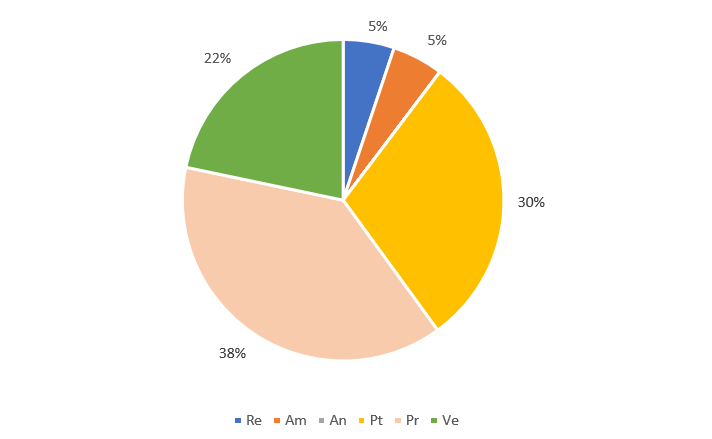
\includegraphics[scale = 0.75]{Immagini/DettaglioTorta.png}
    \caption{Areogramma della ripartizione di ore per ruolo in progettazione di dettaglio e codifica}
    \label{fig:Areogramma ripartizione ore, periodo di Progettazione di Dettaglio e Codifica}
\end{figure}
\newpage
\subsubsection{Specifica dei prospetti}\label{SpecificaPDettaglio}
Per un maggiore controllo sul periodo di progettazione di dettaglio e codifica, vengono di seguito riportati i prospetti orari ed economici suddivisi per le attività individuate nella sezione \S\ref{IncrementiPDettaglio}. Per ogni incremento si riporta inoltre una tabella per tracciare le ore d'impegno previsto per gli obiettivi da raggiungere durante il periodo periodo.
\paragraph{Incremento 1}
\paragraph*{Prospetto orario}
La distribuzione oraria è la seguente:
\begin{table}[H]
	\begin{center}
		\begin{tabular}{ |c c c c c c c c| }
			\rowcolor{darkblue} 
			\textcolor{white}{\textbf{Nominativo}} & \textcolor{white}{\textbf{Re}} & \textcolor{white}{\textbf{Am}} & \textcolor{white}{\textbf{An}} & \textcolor{white}{\textbf{Pt}} & \textcolor{white}{\textbf{Pr}} & \textcolor{white}{\textbf{Ve}} & \textcolor{white}{\textbf{Ore Complessive}} \\ \hline
		\BL 	& 1  	& -  	& - 	& 3 	& 5 	& 3 	& 12 \\ \hline
		\FF 	& -  	& -  	& - 	& 8 	& 4 	& -  	& 12 \\ \hline
		\MM 	& -  	& 2  	& - 	& 3 	& 3 	& 4 	& 12 \\ \hline
		\PC 	& 2 	& 2  	& - 	& 2 	& 3 	& 3 	& 12 \\ \hline
		\TG 	& 2  	& 2		& - 	& 3 	& 3 	& 2 	& 12 \\ \hline
		\TL 	& -  	& - 	& - 	& 5 	& 5 	& 2 	& 12 \\ \hline
		\VD 	& -  	& -  	& - 	& 4 	& 5 	& 3 	& 12 \\ \hline
		\textbf{Ore totali} & \textbf{5} & \textbf{6} & \textbf{-} & \textbf{28} & \textbf{28} & \textbf{17} & \textbf{84} \\ \hline
		\end{tabular}
		\caption{Distribuzione delle ore}
	\end{center}
\end{table}
\paragraph*{Prospetto economico}
Il costo per ogni ruolo è il seguente:
\begin{table}[H]
	\begin{center}
		\begin{tabular}{ |c c c| }
			\rowcolor{darkblue} 
			\textcolor{white}{\textbf{Ruolo}} & \textcolor{white}{\textbf{Ore}} & \textcolor{white}{\textbf{Costo in €}}\\ \hline
		{\Responsabile} 			& 5 	& 150 \\ \hline
		{\Amministratore}		 	& 6 	& 120 \\ \hline
		\textit{Analista} 			& - 	& - \\ \hline
		\textit{Progettista} 		& 28 	& 616 \\ \hline
		\textit{Programmatore}  	& 28 	& 420 \\ \hline
		\textit{Verificatore} 		& 17 	& 255 \\ \hline
		\textbf{Totale} & \textbf{84} & \textbf{1561} \\ \hline
		\end{tabular}
		\caption{Prospetto dei costi per ruoli}
	\end{center}
\end{table}
\paragraph*{Tracciamento obiettivi-ore}
Le ore da impiegare previste per ogni obiettivo sono le seguenti:
\begin{table}[H]
	\begin{center}
		\begin{tabular}{ |c c| }
			\rowcolor{darkblue} 
			\textcolor{white}{\textbf{Obiettivo}}	& \textcolor{white}{\textbf{Ore per il raggiungimento}} \\ \hline
			{Miglioramento documentazione} 			& 14 	\\ \hline
			{Analisi design pattern} 				& 30 	\\ \hline
			{Analisi diagrammi delle classi} 		& 20 	\\ \hline
			{Analisi diagrammi sequenza} 			& 20 	\\ \hline
			\textbf{Totale} 						& \textbf{84}  \\ \hline
		\end{tabular}
		\caption{Tracciamento obiettivo-ore da impiegare Incremento 1}
	\end{center}
\end{table}
\paragraph{Incremento 2}
\paragraph*{Prospetto orario}
La distribuzione oraria è la seguente:
\begin{table}[H]
	\begin{center}
		\begin{tabular}{ |c c c c c c c c| }
			\rowcolor{darkblue} 
			\textcolor{white}{\textbf{Nominativo}} & \textcolor{white}{\textbf{Re}} & \textcolor{white}{\textbf{Am}} & \textcolor{white}{\textbf{An}} & \textcolor{white}{\textbf{Pt}} & \textcolor{white}{\textbf{Pr}} & \textcolor{white}{\textbf{Ve}} & \textcolor{white}{\textbf{Ore Complessive}} \\ \hline
			\BL 	& 1  	& -  	& - 	& 4 	& 5 	& 3 	& 13 \\ \hline
			\FF 	& -  	& -  	& - 	& 8 	& 5 	& -  	& 13 \\ \hline
			\MM 	& -  	& 2  	& - 	& 3 	& 3 	& 5 	& 13 \\ \hline
			\PC 	& 2 	& 2  	& - 	& 2		& 4 	& 3 	& 13 \\ \hline
			\TG 	& 2  	& -		& - 	& 2 	& 6 	& 3 	& 13 \\ \hline
			\TL 	& -  	& - 	& - 	& 2 	& 4 	& 7 	& 13 \\ \hline
			\VD 	& -  	& -  	& - 	& 5 	& 5 	& 3 	& 13 \\ \hline
			\textbf{Ore totali} & \textbf{5} & \textbf{4} & \textbf{-} & \textbf{26} & \textbf{32} & \textbf{24} & \textbf{91} \\ \hline
		\end{tabular}
		\caption{Distribuzione delle ore}
	\end{center}
\end{table}
\paragraph*{Prospetto economico}
Il costo per ogni ruolo è il seguente:
\begin{table}[H]
	\begin{center}
		\begin{tabular}{ |c c c| }
		\rowcolor{darkblue} 
		\textcolor{white}{\textbf{Ruolo}} & \textcolor{white}{\textbf{Ore}} & \textcolor{white}{\textbf{Costo in €}}\\ \hline
		{\Responsabile} 			& 5 	& 150 \\ \hline
		{\Amministratore}		 	& 4 	& 80 \\ \hline
		\textit{Analista} 			& - 	& - \\ \hline
		\textit{Progettista} 		& 26 	& 572 \\ \hline
		\textit{Programmatore}  	& 32 	& 480 \\ \hline
		\textit{Verificatore} 		& 24 	& 360 \\ \hline
		\textbf{Totale} & \textbf{91} & \textbf{1642} \\ \hline
		\end{tabular}
		\caption{Prospetto dei costi per ruoli}
	\end{center}
\end{table}
\paragraph*{Tracciamento obiettivi-ore}
Le ore da impiegare previste per ogni obiettivo sono le seguenti:
\begin{table}[H]
	\begin{center}
		\begin{tabular}{ |c c| }
			\rowcolor{darkblue} 
			\textcolor{white}{\textbf{Obiettivo}}	& \textcolor{white}{\textbf{Ore per il raggiungimento}} \\ \hline
			{Correzione documentazione} 			& 10 	\\ \hline
			{Sviluppo requisiti dominio Utente} 	& 55 	\\ \hline
			{Sviluppo requisiti dominio Prodotti} 	& 26 	\\ \hline
			\textbf{Totale} 						& \textbf{91}  \\ \hline
		\end{tabular}
		\caption{Tracciamento obiettivo-ore da impiegare Incremento 2}
	\end{center}
\end{table}
\paragraph{Incremento 3}
\paragraph*{Prospetto orario}
La distribuzione oraria è la seguente:
\begin{table}[H]
	\begin{center}
		\begin{tabular}{ |c c c c c c c c| }
		\rowcolor{darkblue} 
		\textcolor{white}{\textbf{Nominativo}} & \textcolor{white}{\textbf{Re}} & \textcolor{white}{\textbf{Am}} & \textcolor{white}{\textbf{An}} & \textcolor{white}{\textbf{Pt}} & \textcolor{white}{\textbf{Pr}} & \textcolor{white}{\textbf{Ve}} & \textcolor{white}{\textbf{Ore Complessive}} \\ \hline
		\BL 	& 1  	& -  	& - 	& 4 	& 6 	& 2 	& 13 \\ \hline
		\FF 	& -  	& -  	& - 	& 10 	& 3 	& -  	& 13 \\ \hline
		\MM 	& -  	& 2  	& - 	& 6 	& 3 	& 2 	& 13 \\ \hline
		\PC 	& 1 	& -  	& - 	& 4 	& 5 	& 3 	& 13 \\ \hline
		\TG 	& 1  	& -		& - 	& 1 	& 4 	& 7 	& 13 \\ \hline
		\TL 	& -  	& - 	& - 	& 5 	& 5 	& 3 	& 13 \\ \hline
		\VD 	& 1  	& 1  	& - 	& 2 	& 5 	& 4 	& 13 \\ \hline
		\textbf{Ore totali} & \textbf{4} & \textbf{3} & \textbf{-} & \textbf{32} & \textbf{31} & \textbf{21} & \textbf{91} \\ \hline
		\end{tabular}
		\caption{Distribuzione delle ore}
	\end{center}
\end{table}
\paragraph*{Prospetto economico}
Il costo per ogni ruolo è il seguente:
\begin{table}[H]
	\begin{center}
		\begin{tabular}{ |c c c| }
			\rowcolor{darkblue} 
			\textcolor{white}{\textbf{Ruolo}} & \textcolor{white}{\textbf{Ore}} & \textcolor{white}{\textbf{Costo in €}}\\ \hline
		{\Responsabile} 			& 4 	& 120 \\ \hline
		{\Amministratore}		 	& 3 	& 60 \\ \hline
		\textit{Analista} 			& - 	& - \\ \hline
		\textit{Progettista} 		& 32 	& 704 \\ \hline
		\textit{Programmatore}  	& 31 	& 465 \\ \hline
		\textit{Verificatore} 		& 21 	& 315 \\ \hline
		\textbf{Totale} & \textbf{91} & \textbf{1664} \\ \hline
		\end{tabular}
		\caption{Prospetto dei costi per ruoli}
	\end{center}
\end{table}
\paragraph*{Tracciamento obiettivi-ore}
Le ore da impiegare previste per ogni obiettivo sono le seguenti:
\begin{table}[H]
	\begin{center}
		\begin{tabular}{ |c c| }
			\rowcolor{darkblue} 
			\textcolor{white}{\textbf{Obiettivo}}	& \textcolor{white}{\textbf{Ore per il raggiungimento}} \\ \hline
			{Sviluppo requisiti dominio Prodotti} 	& 51 	\\ \hline
			{Sviluppo requisiti dominio Carrello} 	& 30 	\\ \hline
			{Preparazione alla \glo{PB}} 			&  10	\\ \hline
			\textbf{Totale} 						& \textbf{91}  \\ \hline
		\end{tabular}
		\caption{Tracciamento obiettivo-ore da impiegare Incremento 3}
	\end{center}
\end{table}
\paragraph{Incremento 4}
\paragraph*{Prospetto orario}
La distribuzione oraria è la seguente:
\begin{table}[H]
	\begin{center}
		\begin{tabular}{ |c c c c c c c c| }
			\rowcolor{darkblue} 
			\textcolor{white}{\textbf{Nominativo}} & \textcolor{white}{\textbf{Re}} & \textcolor{white}{\textbf{Am}} & \textcolor{white}{\textbf{An}} & \textcolor{white}{\textbf{Pt}} & \textcolor{white}{\textbf{Pr}} & \textcolor{white}{\textbf{Ve}} & \textcolor{white}{\textbf{Ore Complessive}} \\ \hline
			\BL 	& 1  	& -  	& - 	& 4 	& 5 	& 2 	& 12 \\ \hline
			\FF 	& -  	& -  	& - 	& 4 	& 8 	& -  	& 12 \\ \hline
			\MM 	& -  	& 2  	& - 	& 3 	& 5 	& 2 	& 12 \\ \hline
			\PC 	& - 	& -  	& - 	& 3 	& 6 	& 3 	& 12 \\ \hline
			\TG 	& -  	& -		& - 	& - 	& 7 	& 5 	& 12 \\ \hline
			\TL 	& -  	& - 	& - 	& 3 	& 6 	& 3 	& 12 \\ \hline
			\VD 	& 3  	& 3  	& - 	& 1 	& 5 	& -		& 12 \\ \hline
			\textbf{Ore totali} & \textbf{4} & \textbf{5} & \textbf{-} & \textbf{18} & \textbf{42} & \textbf{15} & \textbf{84} \\ \hline
		\end{tabular}
		\caption{Distribuzione delle ore}
	\end{center}
\end{table}
\paragraph*{Prospetto economico}
Il costo per ogni ruolo è il seguente:
\begin{table}[H]
	\begin{center}
		\begin{tabular}{ |c c c| }
			\rowcolor{darkblue} 
			\textcolor{white}{\textbf{Ruolo}} & \textcolor{white}{\textbf{Ore}} & \textcolor{white}{\textbf{Costo in €}}\\ \hline
		{\Responsabile} 			& 4 	& 120 \\ \hline
		{\Amministratore}		 	& 5 	& 100 \\ \hline
		\textit{Analista} 			& - 	& - \\ \hline
		\textit{Progettista} 		& 18 	& 396 \\ \hline
		\textit{Programmatore}  	& 42 	& 630 \\ \hline
		\textit{Verificatore} 		& 15 	& 225 \\ \hline
		\textbf{Totale} & \textbf{84} & \textbf{1471} \\ \hline
		\end{tabular}
		\caption{Prospetto dei costi per ruoli}
	\end{center}
\end{table}
\paragraph*{Tracciamento obiettivi-ore}
Le ore da impiegare previste per ogni obiettivo sono le seguenti:
\begin{table}[H]
	\begin{center}
		\begin{tabular}{ |c c| }
			\rowcolor{darkblue} 
			\textcolor{white}{\textbf{Obiettivo}}	& \textcolor{white}{\textbf{Ore per il raggiungimento}} \\ \hline
			{Redazione manuali} 					& 10 	\\ \hline
			{Sviluppo requisiti dominio Servizio Pagamento}&  19	\\ \hline
			{Sviluppo requisiti dominio Ordini} 	& 45 	\\ \hline
			{Preparazione alla \glo{RQ}} 			& 10 	\\ \hline
			\textbf{Totale} 						& \textbf{84}  \\ \hline
		\end{tabular}
		\caption{Tracciamento obiettivo-ore da impiegare Incremento 4}
	\end{center}
\end{table}
\subsection{Periodo di validazione e collaudo}
\subsubsection{Prospetto orario}
In questo periodo la distribuzione oraria è la seguente:
\begin{table}[H]
	\begin{center}
		\begin{tabular}{ |c c c c c c c c| }
		\rowcolor{darkblue} 
		\textcolor{white}{\textbf{Nominativo}} & \textcolor{white}{\textbf{Re}} & \textcolor{white}{\textbf{Am}} & \textcolor{white}{\textbf{An}} & \textcolor{white}{\textbf{Pt}} & \textcolor{white}{\textbf{Pr}} & \textcolor{white}{\textbf{Ve}} & \textcolor{white}{\textbf{Ore Complessive}} \\ \hline
		\BL 	& -  	& 5  	& - 	& 5 	& - 	& 10 	& 20 \\ \hline
		\FF 	& 4  	& 5  	& - 	& - 	& 5 	& 6  	& 20 \\ \hline
		\MM 	& 4 	& - 	& - 	& - 	& 6 	& 10  	& 20 \\ \hline
		\PC 	& 5 	& -  	& - 	& - 	& 7 	& 8 	& 20 \\ \hline
		\TG 	& -  	& 6 	& - 	& - 	& 8 	& 6 	& 20 \\ \hline
		\TL 	& -  	& - 	& - 	& 4 	& 6 	& 10 	& 20 \\ \hline
		\VD 	& 4  	& -  	& - 	& - 	& 4 	& 12  	& 20 \\ \hline
		\textbf{Ore totali} & \textbf{17} & \textbf{16} & \textbf{-} & \textbf{9} & \textbf{36} & \textbf{62} & \textbf{140} \\ \hline
		\end{tabular}
	\caption{Distribuzione delle ore nel periodo di validazione e collaudo}
	\end{center}
\end{table}
I dati ottenuti vengono riassunti nel seguente istogramma:
\begin{figure}[H]
    \centering
    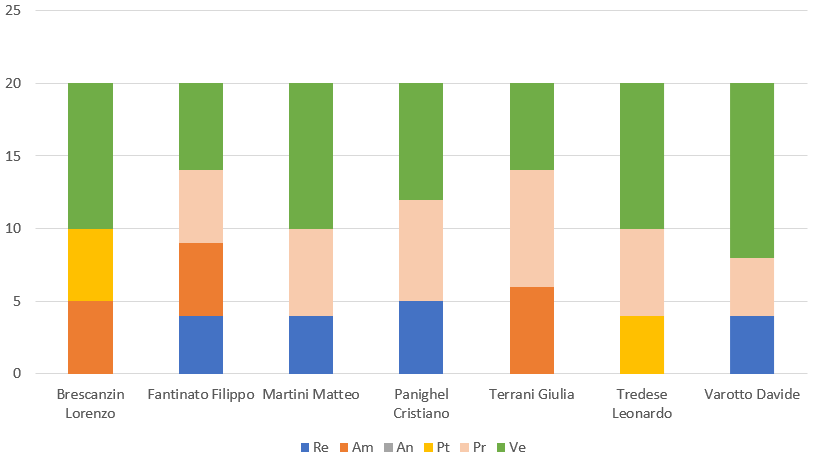
\includegraphics[scale = 0.70]{Immagini/ValidazioneIsto.png}
    \caption{Istogramma della ripartizione delle ore per ruolo in validazione e collaudo}
    \label{fig:istogramma ripartizione ore, periodo di Validazione e Collaudo}
\end{figure}
\newpage
\subsubsection{Prospetto economico}
Il costo per ogni ruolo è il seguente:
\begin{table}[H]
	\begin{center}
		\begin{tabular}{ |c c c| }
		\rowcolor{darkblue} 
		\textcolor{white}{\textbf{Ruolo}} & \textcolor{white}{\textbf{Ore}} & \textcolor{white}{\textbf{Costo in €}}\\ \hline
		{\Responsabile} 			& 17 	& 510 \\ \hline
		{\Amministratore}		 	& 16 	& 320 \\ \hline
		\textit{Analista} 			& - 	& - \\ \hline
		\textit{Progettista} 		& 9 	& 198 \\ \hline
		\textit{Programmatore}  	& 36 	& 540 \\ \hline
		\textit{Verificatore} 		& 62 	& 930 \\ \hline
		\textbf{Totale} & \textbf{140} & \textbf{2498} \\ \hline
		\end{tabular}
	\caption{Prospetto dei costi per ruoli nel periodo di validazione e collaudo}
	\end{center}
\end{table}
Il seguente grafico a torta riassume i dati ottenuti:
\begin{figure}[H]
    \centering
    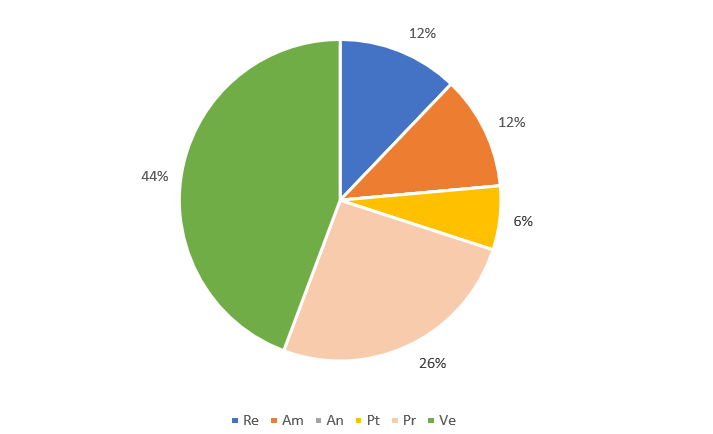
\includegraphics[scale = 0.75]{Immagini/ValidazioneTorta.png}
    \caption{Areogramma della ripartizione di ore per ruolo in validazione e collaudo}
    \label{fig:Areogramma ripartizione ore, periodo di Validazione e Collaudo}
\end{figure}
\subsubsection{Rimodulazione del volume d'impegno}\label{RimodulazioneOre}
A causa dei ritardi avuti durante i precedenti periodi, per poter rispettare il preventivo concordato durante la \glo{RR}, si è dovuto procedere ad una rimodulazione dell'impegno orario da impiegare.
Si è ritenuto ragionevole modificare le ore di lavoro previste per questo periodo ritenendo che le ore pianificate per il periodo di progettazione di dettaglio e collaudo individuate siano necessarie per poter creare un prodotto solido che durante il periodo di validazione verrà solo raffinato. Di seguito si riportano i prospetti, orario ed economico, considerati esclusivamente in relazione con i valori del consutivo ottenuti nei precedenti periodi.
\subsubsection{Prospetto orario}
In questo periodo la distribuzione oraria è la seguente:
\begin{table}[H]
	\begin{center}
		\begin{tabular}{ |c c c c c c c c| }
			\rowcolor{darkblue} 
			\textcolor{white}{\textbf{Nominativo}} & \textcolor{white}{\textbf{Re}} & \textcolor{white}{\textbf{Am}} & \textcolor{white}{\textbf{An}} & \textcolor{white}{\textbf{Pt}} & \textcolor{white}{\textbf{Pr}} & \textcolor{white}{\textbf{Ve}} & \textcolor{white}{\textbf{Ore Complessive}} \\ \hline
			\BL 	& -  	& 4  	& - 	& 4 	& - 	& 10 	& 18 \\ \hline
			\FF 	& 3  	& 4  	& - 	& - 	& 4 	& 7  	& 18 \\ \hline
			\MM 	& 4 	& - 	& - 	& - 	& 4 	& 10  	& 18 \\ \hline
			\PC 	& 4 	& -  	& - 	& - 	& 6 	& 8 	& 18 \\ \hline
			\TG 	& -  	& 4 	& - 	& - 	& 7 	& 7 	& 18 \\ \hline
			\TL 	& -  	& - 	& - 	& 4 	& 4 	& 10 	& 18 \\ \hline
			\VD 	& 3  	& -  	& - 	& - 	& 3 	& 12  	& 18 \\ \hline
			\textbf{Ore totali} & \textbf{14} & \textbf{12} & \textbf{-} & \textbf{8} & \textbf{28} & \textbf{64} & \textbf{126} \\ \hline
		\end{tabular}
		\caption{Distribuzione delle ore nel periodo di validazione e collaudo}
	\end{center}
\end{table}
\subsubsection{Prospetto economico}
Il costo per ogni ruolo è il seguente:
\begin{table}[H]
	\begin{center}
		\begin{tabular}{ |c c c| }
			\rowcolor{darkblue} 
			\textcolor{white}{\textbf{Ruolo}} & \textcolor{white}{\textbf{Ore}} & \textcolor{white}{\textbf{Costo in €}}\\ \hline
			{\Responsabile} 			& 14 	& 420 \\ \hline
			{\Amministratore}		 	& 12 	& 240 \\ \hline
			\textit{Analista} 			& - 	& - \\ \hline
			\textit{Progettista} 		& 8 	& 176 \\ \hline
			\textit{Programmatore}  	& 28 	& 420 \\ \hline
			\textit{Verificatore} 		& 64 	& 960 \\ \hline
			\textbf{Totale} & \textbf{126} & \textbf{2216} \\ \hline
		\end{tabular}
		\caption{Prospetto dei costi per ruoli nel periodo di validazione e collaudo}
	\end{center}
\end{table}
\subsubsection{Specifica dei prospetti}\label{SpecificaValidazione}
Per un maggiore controllo sul periodo di validazione e collaudo, vengono di seguito riportati i prospetti orari ed economici suddivisi per le attività individuate nella sezione \S\ref{IncrementiValidazione}. Per ogni incremento si riporta inoltre una tabella per tracciare le ore d'impegno previsto per gli obiettivi da raggiungere durante il periodo periodo.
\paragraph{Incremento 1}
\paragraph*{Prospetto orario}
La distribuzione oraria è la seguente:
\begin{table}[H]
	\begin{center}
		\begin{tabular}{ |c c c c c c c c| }
			\rowcolor{darkblue} 
			\textcolor{white}{\textbf{Nominativo}} & \textcolor{white}{\textbf{Re}} & \textcolor{white}{\textbf{Am}} & \textcolor{white}{\textbf{An}} & \textcolor{white}{\textbf{Pt}} & \textcolor{white}{\textbf{Pr}} & \textcolor{white}{\textbf{Ve}} & \textcolor{white}{\textbf{Ore Complessive}} \\ \hline
			\BL 	& -  	& 4  	& - 	& 4 	& - 	& 5 	& 13 \\ \hline
			\FF 	& 3  	& 3  	& - 	& - 	& 3 	& 4  	& 13 \\ \hline
			\MM 	& 3 	& - 	& - 	& - 	& 4 	& 6 	& 13 \\ \hline
			\PC 	& 2 	& -  	& - 	& - 	& 4 	& 7 	& 13 \\ \hline
			\TG 	& -  	& 4 	& - 	& - 	& 5 	& 4 	& 13 \\ \hline
			\TL 	& -  	& - 	& - 	& 4 	& 4 	& 5 	& 13 \\ \hline
			\VD 	& 3  	& -  	& - 	& - 	& 3 	& 7  	& 13 \\ \hline
			\textbf{Ore totali} & \textbf{11} & \textbf{11} & \textbf{-} & \textbf{8} & \textbf{23} & \textbf{38} & \textbf{91} \\ \hline
		\end{tabular}
		\caption{Distribuzione delle ore nel periodo di validazione e collaudo}
	\end{center}
\end{table}
\paragraph*{Prospetto economico}
Il costo per ogni ruolo è il seguente:
\begin{table}[H]
	\begin{center}
		\begin{tabular}{ |c c c| }
			\rowcolor{darkblue} 
			\textcolor{white}{\textbf{Ruolo}} & \textcolor{white}{\textbf{Ore}} & \textcolor{white}{\textbf{Costo in €}}\\ \hline
			{\Responsabile} 			& 11 	& 330 \\ \hline
			{\Amministratore}		 	& 11 	& 220 \\ \hline
			\textit{Analista} 			& - 	& - \\ \hline
			\textit{Progettista} 		& 8 	& 176 \\ \hline
			\textit{Programmatore}  	& 23 	& 345 \\ \hline
			\textit{Verificatore} 		& 38 	& 570 \\ \hline
			\textbf{Totale} & \textbf{91} & \textbf{1641} \\ \hline
		\end{tabular}
		\caption{Prospetto dei costi per ruoli nel periodo di validazione e collaudo}
	\end{center}
\end{table}
\paragraph*{Tracciamento obiettivi-ore}
Le ore da impiegare previste per ogni obiettivo sono le seguenti:
\begin{table}[H]
	\begin{center}
		\begin{tabular}{ |c c| }
			\rowcolor{darkblue} 
			\textcolor{white}{\textbf{Obiettivo}}	& \textcolor{white}{\textbf{Ore per il raggiungimento}} \\ \hline
			{Sviluppo ultimi requisiti domini precedenti} 	& 17 	\\ \hline
			{Sviluppo requisiti dominio Ordini} 	& 54 	\\ \hline
			{Correzione documentazione} 			&  20	\\ \hline
			\textbf{Totale} 						& \textbf{91}  \\ \hline
		\end{tabular}
		\caption{Tracciamento obiettivo-ore da impiegare Incremento 1}
	\end{center}
\end{table}
\paragraph{Incremento 2}
\paragraph*{Prospetto orario}
La distribuzione oraria è la seguente:
\begin{table}[H]
	\begin{center}
		\begin{tabular}{ |c c c c c c c c| }
			\rowcolor{darkblue} 
			\textcolor{white}{\textbf{Nominativo}} & \textcolor{white}{\textbf{Re}} & \textcolor{white}{\textbf{Am}} & \textcolor{white}{\textbf{An}} & \textcolor{white}{\textbf{Pt}} & \textcolor{white}{\textbf{Pr}} & \textcolor{white}{\textbf{Ve}} & \textcolor{white}{\textbf{Ore Complessive}} \\ \hline
			\BL 	& -  	& -  	& - 	& - 	& - 	& 5 	& 5 \\ \hline
			\FF 	& -  	& 1  	& - 	& - 	& 1 	& 3  	& 5 \\ \hline
			\MM 	& 1 	& - 	& - 	& - 	& - 	& 4  	& 5 \\ \hline
			\PC 	& 2 	& -  	& - 	& - 	& 2 	& 1 	& 5 \\ \hline
			\TG 	& -  	& - 	& - 	& - 	& 2 	& 3 	& 5 \\ \hline
			\TL 	& -  	& - 	& - 	& - 	& - 	& 5 	& 5 \\ \hline
			\VD 	& -  	& -  	& - 	& - 	& - 	& 5  	& 5 \\ \hline
			\textbf{Ore totali} & \textbf{3} & \textbf{1} & \textbf{-} & \textbf{-} & \textbf{5} & \textbf{26} & \textbf{35} \\ \hline
		\end{tabular}
		\caption{Distribuzione delle ore nel periodo di validazione e collaudo}
	\end{center}
\end{table}
\paragraph*{Prospetto economico}
Il costo per ogni ruolo è il seguente:
\begin{table}[H]
	\begin{center}
		\begin{tabular}{ |c c c| }
			\rowcolor{darkblue} 
			\textcolor{white}{\textbf{Ruolo}} & \textcolor{white}{\textbf{Ore}} & \textcolor{white}{\textbf{Costo in €}}\\ \hline
			{\Responsabile} 			& 3 	& 90 \\ \hline
			{\Amministratore}		 	& 1 	& 20 \\ \hline
			\textit{Analista} 			& - 	& - \\ \hline
			\textit{Progettista} 		& -	& - \\ \hline
			\textit{Programmatore}  	& 5 	& 75 \\ \hline
			\textit{Verificatore} 		& 26 	& 390 \\ \hline
			\textbf{Totale} & \textbf{35} & \textbf{575} \\ \hline
		\end{tabular}
		\caption{Prospetto dei costi per ruoli nel periodo di validazione e collaudo}
	\end{center}
\end{table}
\newpage

\subsection{Riepilogo}
\subsubsection{Ore totali}
\myparagraph{Suddivisione del lavoro}
Nella seguente tabella vengono riportate il totale delle ore del progetto, sono presenti sia le ore di investimento, sia le ore rendicontate a carico del committente.
\begin{table}[H]
	\begin{center}
		\begin{tabular}{ |c c c c c c c c| }
		\rowcolor{darkblue} 
		\textcolor{white}{\textbf{Nominativo}} & \textcolor{white}{\textbf{Re}} & \textcolor{white}{\textbf{Am}} & \textcolor{white}{\textbf{An}} & \textcolor{white}{\textbf{Pt}} & \textcolor{white}{\textbf{Pr}} & \textcolor{white}{\textbf{Ve}} & \textcolor{white}{\textbf{Ore Complessive}} \\ \hline
		\BL 	& 4  	& 14  	& 24 	& 35 	& 24 	& 35 	& 136 \\ \hline
		\FF 	& 7 	& 13 	& 18 	& 46 	& 30 	& 22 	& 136 \\ \hline
		\MM 	& 19  	& 11  	& 22 	& 23 	& 26 	& 35  	& 136 \\ \hline
		\PC 	& 15 	& 8  	& 24 	& 13 	& 29	& 47 	& 136 \\ \hline
		\TG 	& 7  	& 26 	& 24 	& 19 	& 28 	& 32 	& 136 \\ \hline
		\TL 	& 12  	& 11 	& 16 	& 19 	& 30 	& 48 	& 136 \\ \hline
		\VD 	& 18  	& 12  	& 16 	& 26 	& 24 	& 40 	& 136 \\ \hline
		\textbf{Ore totali} & \textbf{82} & \textbf{95} & \textbf{144} & \textbf{181} & \textbf{191} & \textbf{259} & \textbf{952} \\ \hline
		\end{tabular}
	\caption{Distribuzione delle ore totali di investimento e rendicontate}
	\end{center}
\end{table}
I dati ottenuti vengono riassunti nel seguente istogramma:
\begin{figure}[H]
    \centering
    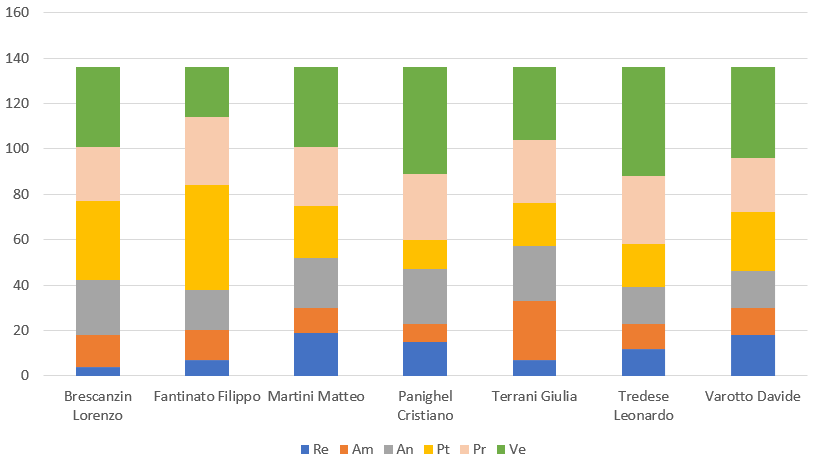
\includegraphics[scale = 0.70]{Immagini/TotaleIsto.png}
    \caption{Istogramma della ripartizione delle ore totali di investimento e rendicontate}
    \label{fig:Istogramma ripartizione ore totali di investimento e rendicontate }
\end{figure}
\newpage
\myparagraph{Prospetto economico}
Il costo per ogni ruolo è il seguente:
\begin{table}[H]
	\begin{center}
		\begin{tabular}{ |c c c| }
		\rowcolor{darkblue} 
		\textcolor{white}{\textbf{Ruolo}} & \textcolor{white}{\textbf{Ore}} & \textcolor{white}{\textbf{Costo in €}}\\ \hline
		{\Responsabile} 			& 82 	& 2460 \\ \hline
		{\Amministratore} 			& 95 	& 1900 \\ \hline
		\textit{Analista} 			& 144 	& 3600 \\ \hline
		\textit{Progettista} 		& 181 	& 3982 \\ \hline
		\textit{Programmatore}  	& 191 	& 2865 \\ \hline
		\textit{Verificatore} 		& 259 	& 3885 \\ \hline
		\textbf{Totale} & \textbf{952} & \textbf{18692} \\  \hline
		\end{tabular}
	\caption{Prospetto delle ore totali di investimento e rendicontate}
	\end{center}
\end{table}
Il seguente grafico a torta riassume i dati ottenuti:
\begin{figure}[H]
    \centering
    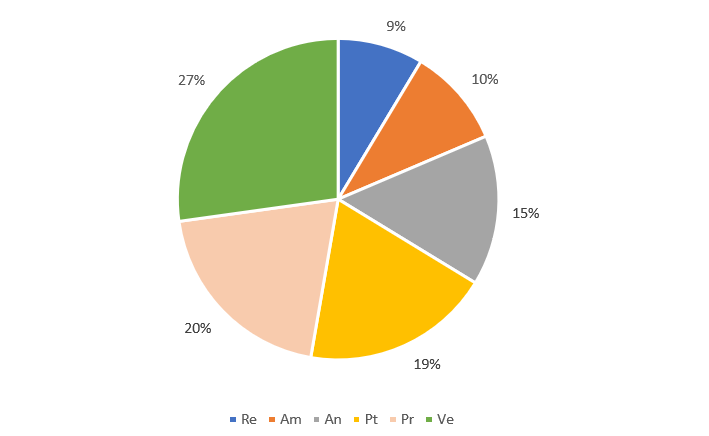
\includegraphics[scale = 0.75]{Immagini/TotaleTorta.png}
    \caption{ Areogramma dei costi totale delle ore di investimento e rendicontate}
    \label{fig:areogramma ripartizione ore totali di investimento e rendicontate}
\end{figure}
\newpage

\subsubsection{Ore rendicontate}
\myparagraph{Suddivisione del lavoro}
Nella seguente tabella sono riassunte le ore rendicontate prima della rimodulazione oraria effettuata per il periodo di validazione e collaudo indicata nella sezione \S\ref{RipianificazioneValidazione}. Le ore rendicontate con la rimodulazione del periodo di validazione è pari a 98 per ciascun componente, si ritiene comunque opportuno presentare la suddivisione oraria stabilita dal preventivo iniziale in quanto la rimodulazione deve essere considerata solo in relazione ai risultati del consuntivo.
\begin{table}[H]
	\begin{center}
		\begin{tabular}{ |c c c c c c c c| }
		\rowcolor{darkblue} 
		\textcolor{white}{\textbf{Nominativo}} & \textcolor{white}{\textbf{Re}} & \textcolor{white}{\textbf{Am}} & \textcolor{white}{\textbf{An}} & \textcolor{white}{\textbf{Pt}} & \textcolor{white}{\textbf{Pr}} & \textcolor{white}{\textbf{Ve}} & \textcolor{white}{\textbf{Ore Complessive}} \\ \hline
		\BL 	& 4  	& 5  	& 8 	& 32 	& 24 	& 27 	& 100 \\ \hline
		\FF 	& 7 	& 5 	& -		& 46 	& 30 	& 12 	& 100 \\ \hline
		\MM 	& 4  	& 11  	& 10 	& 23 	& 26 	& 26  	& 100 \\ \hline
		\PC 	& 10 	& 4  	& 10	& 11 	& 29	& 36 	& 100 \\ \hline
		\TG 	& 5  	& 11 	& 10 	& 19 	& 28 	& 27 	& 100 \\ \hline
		\TL 	& 5  	& 6 	& - 	& 19 	& 32 	& 38 	& 100 \\ \hline
		\VD 	& 18  	& 12  	& -		& 24 	& 24 	& 22 	& 100 \\ \hline
		\textbf{Ore totali} & \textbf{53} & \textbf{54} & \textbf{38} & \textbf{174} & \textbf{193} & \textbf{188} & \textbf{700} \\ \hline
	\end{tabular}
	\caption{Distribuzione delle ore rendicontate}
	\end{center}
\end{table}
I dati ottenuti vengono riassunti nel seguente istogramma:
\begin{figure}[H]
    \centering
    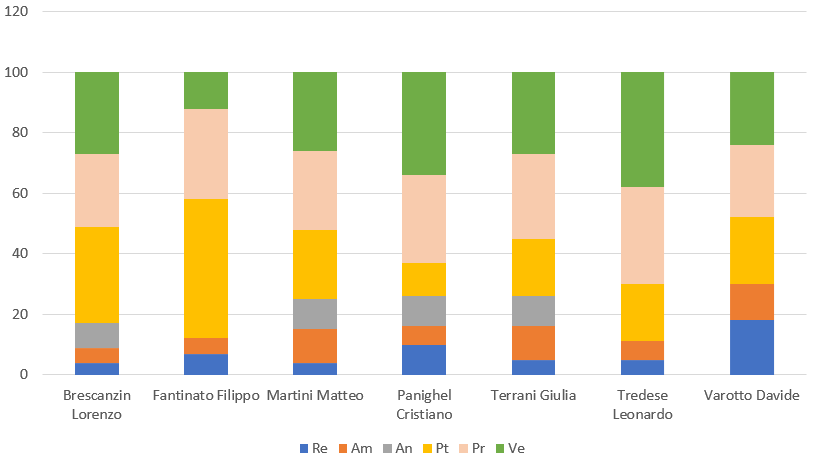
\includegraphics[scale = 0.70]{Immagini/TotaleRendicontatoIsto.png}
    \caption{Istogramma della ripartizione delle ore rendicontate}
    \label{fig:Istogramma ripartizione ore totali rendicontate}
\end{figure}
\newpage
\myparagraph{Prospetto economico}
Il costo totale rendicontato per ogni ruolo è il seguente:
\begin{table}[H]
	\begin{center}
		\begin{tabular}{ |c c c| }
		\rowcolor{darkblue} 
		\textcolor{white}{\textbf{Ruolo}} & \textcolor{white}{\textbf{Ore}} & \textcolor{white}{\textbf{Costo in €}}\\ \hline
		{\Responsabile} 			& 53 	& 1590 \\ \hline
		{\Amministratore}			& 54 	& 1080 \\ \hline
		\textit{Analista} 			& 38 	& 950 \\ \hline
		\textit{Progettista} 		& 174 	& 3828 \\ \hline
		\textit{Programmatore} 		& 193 	& 2895 \\ \hline
		\textit{Verificatore} 		& 188 	& 2820 \\ \hline
		\textbf{Totale} & \textbf{700} & \textbf{13163} \\ \hline
		\end{tabular}
	\caption{Prospetto delle ore rendicontate}
	\end{center}
\end{table}
Il seguente grafico a torta riassume i dati ottenuti:
\begin{figure}[H]
    \centering
    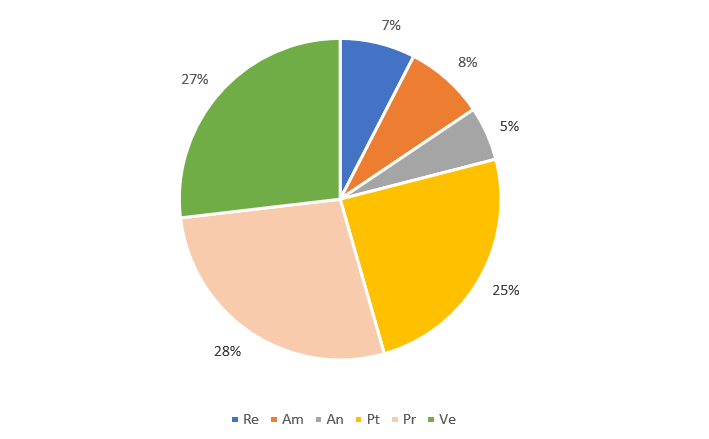
\includegraphics[scale = 0.75]{Immagini/TotaleRendicontatoTorta.png}
    \caption{Areogramma delle ore rendicontate per ruolo}
    \label{fig:Areogramma ripartizione ore totali rendicontate}
\end{figure}
\subsubsection{Conclusioni}
Il costo totale preventivato è: 13163€.